\documentclass[border=10pt]{standalone}
\usepackage{pgfplots}
\usepgfplotslibrary{groupplots}
\pgfplotsset{compat=1.18}
\begin{document}
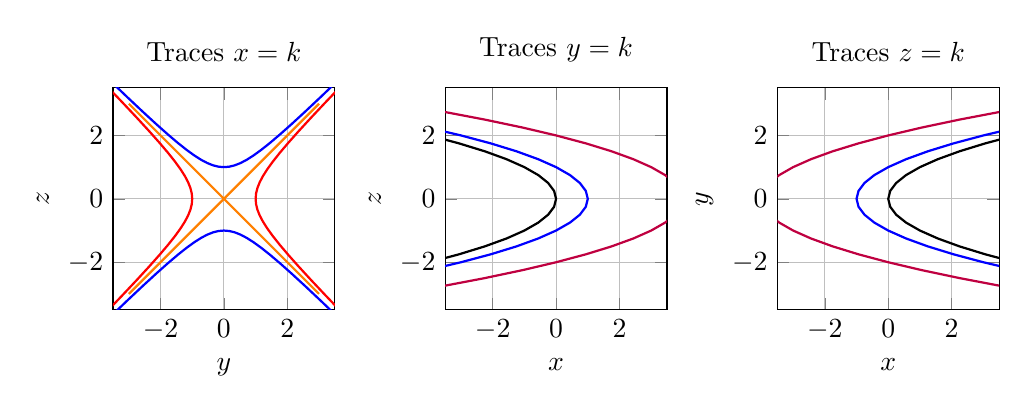
\begin{tikzpicture}
\begin{groupplot}[
    group style={group size=3 by 1, horizontal sep=1.4cm},
    width=5.2cm, height=4.4cm,
    grid=major,
    axis equal image,
    xmin=-3.5, xmax=3.5,
    ymin=-3.5, ymax=3.5
]
\nextgroupplot[xlabel=$y$, ylabel=$z$, title={Traces $x=k$}]
\addplot[domain=-3:3, orange, thick] ({x},{x});
\addplot[domain=-3:3, orange, thick] ({x},{-x});
\addplot[domain=-2:2, red, thick] ({cosh(x)},{sinh(x)});
\addplot[domain=-2:2, red, thick] ({-cosh(x)},{sinh(x)});
\addplot[domain=-2:2, blue, thick] ({sinh(x)},{cosh(x)});
\addplot[domain=-2:2, blue, thick] ({sinh(x)},{-cosh(x)});

\nextgroupplot[xlabel=$x$, ylabel=$z$, title={Traces $y=k$}]
\addplot[domain=-3:3, black, thick] ({-x*x},{x});
\addplot[domain=-3:3, blue, thick] ({1-x*x},{x});
\addplot[domain=-3:3, purple, thick] ({4-x*x},{x});

\nextgroupplot[xlabel=$x$, ylabel=$y$, title={Traces $z=k$}]
\addplot[domain=-3:3, black, thick] ({x*x},{x});
\addplot[domain=-3:3, blue, thick] ({x*x-1},{x});
\addplot[domain=-3:3, purple, thick] ({x*x-4},{x});
\end{groupplot}
\end{tikzpicture}
\end{document}